\documentclass[10pt,letterpaper]{article}
\usepackage[top=0.85in,left=2.75in,footskip=0.75in,marginparwidth=2in]{geometry}

% use Unicode characters - try changing the option if you run into troubles with special characters (e.g. umlauts)

\usepackage[utf8]{inputenc}
\usepackage{listings}


% clean citations
\usepackage{cite}

% hyperref makes references clicky. use \url{www.example.com} or \href{www.example.com}{description} to add a clicky url
\usepackage{nameref,hyperref}

% line numbers
\usepackage[right]{lineno}

% improves typesetting in LaTeX
\usepackage{microtype}
\DisableLigatures[f]{encoding = *, family = * }

% text layout - change as needed
\raggedright
\setlength{\parindent}{0.5cm}
\textwidth 5.25in
\textheight 8.75in

% use adjustwidth environment to exceed text width (see examples in text)
\usepackage{changepage}

% adjust caption style

% remove brackets from references
\makeatletter
\renewcommand{\@biblabel}[1]{\quad#1.}
\makeatother

% headrule, footrule and page numbers
\usepackage{lastpage,fancyhdr,graphicx}
\usepackage{epstopdf}
\pagestyle{myheadings}
\pagestyle{fancy}
\fancyhf{}
\rfoot{\thepage/\pageref{LastPage}}
\renewcommand{\footrule}{\hrule height 2pt \vspace{2mm}}
\fancyheadoffset[L]{2.25in}
\fancyfootoffset[L]{2.25in}

% use \textcolor{color}{text} for colored text (e.g. highlight to-do areas)
\usepackage{color}

% define custom colors (this one is for figure captions)
\definecolor{Gray}{gray}{.25}

% this is required to include graphics
\usepackage{graphicx}

% use if you want to put caption to the side of the figure - see example in text
\usepackage{sidecap}

% use for have text wrap around figures
\usepackage{wrapfig}
\usepackage[pscoord]{eso-pic}
\usepackage[fulladjust]{marginnote}
\reversemarginpar

% document begins here
\begin{document}
\vspace*{0.35in}

% title goes here:
\begin{flushleft}
{\Large
  \textbf\newline{Supplementaries for "pyranges: efficient comparisons of genomic intervals in Python"}
  % and arithmetic run length-encoding
}
\newline
% authors go here:
\\
Endre Bakken Stovner\textsuperscript{1},
Pål Sætrom\textsuperscript{1, 2},
\\
\bf{1} Department of
  Computer Science, Norwegian University
  of Science and Technology, Trondheim, 7013, Norway
\\
\bf{2} Department of Clinical and Molecular Medicine, Norwegian
  University of Science and Technology, Trondheim, 7013, Norway
\\
\bigskip
* endrebak85@gmail.com

\end{flushleft}

\section*{Testing}

To test the PyRanges library, three different types of testing were used.

\subsection*{Unit-testing}

Regular unit tests were written for all functions and their settings. This was
mostly to aid development using test-driven development.

\subsection*{Property-based testing}

To ensure correctness, PyRanges was tested against long-lived, well-tested and
popular libraries that provide the same functionality like bedtools and R
GenomicRanges. PyRanges and these existing libraries were run on tens of
thousands of random examples produced by hypothesis
(https://github.com/HypothesisWorks/hypothesis) to ensure that PyRanges returned
the same result.

In addition to using hypothesis for oracular testing, we also used hypothesis to
ensure that some properties that should always hold (such as inverse operations
on runlengths, like + and - gives the start value as a result) indeed held true.

\subsection*{Testing for memory-leaks}

Valgrind \cite{Nethercote:2007:SBM:1254810.1254820} was used to ensure that the
high-performance C/Cython code did not leak memory.

The memory leakage of different PyRanges functionality (e.g. intersection, rle
division) was measured. The functions were repeated 1, 10, 100 and 1000 times in
a loop so that cumulative effects of potentially small leaks could be detected.
In figure \ref{fig1}, we deducted the initial 0,00015-MB memory leak detected
from importing pandas (which PyRanges depends on) in the results.

\begin{figure}
% the number in [] of wrapfigure is optional and gives the number of text lines that should be wrapped around the text. Adjust according to your figures height
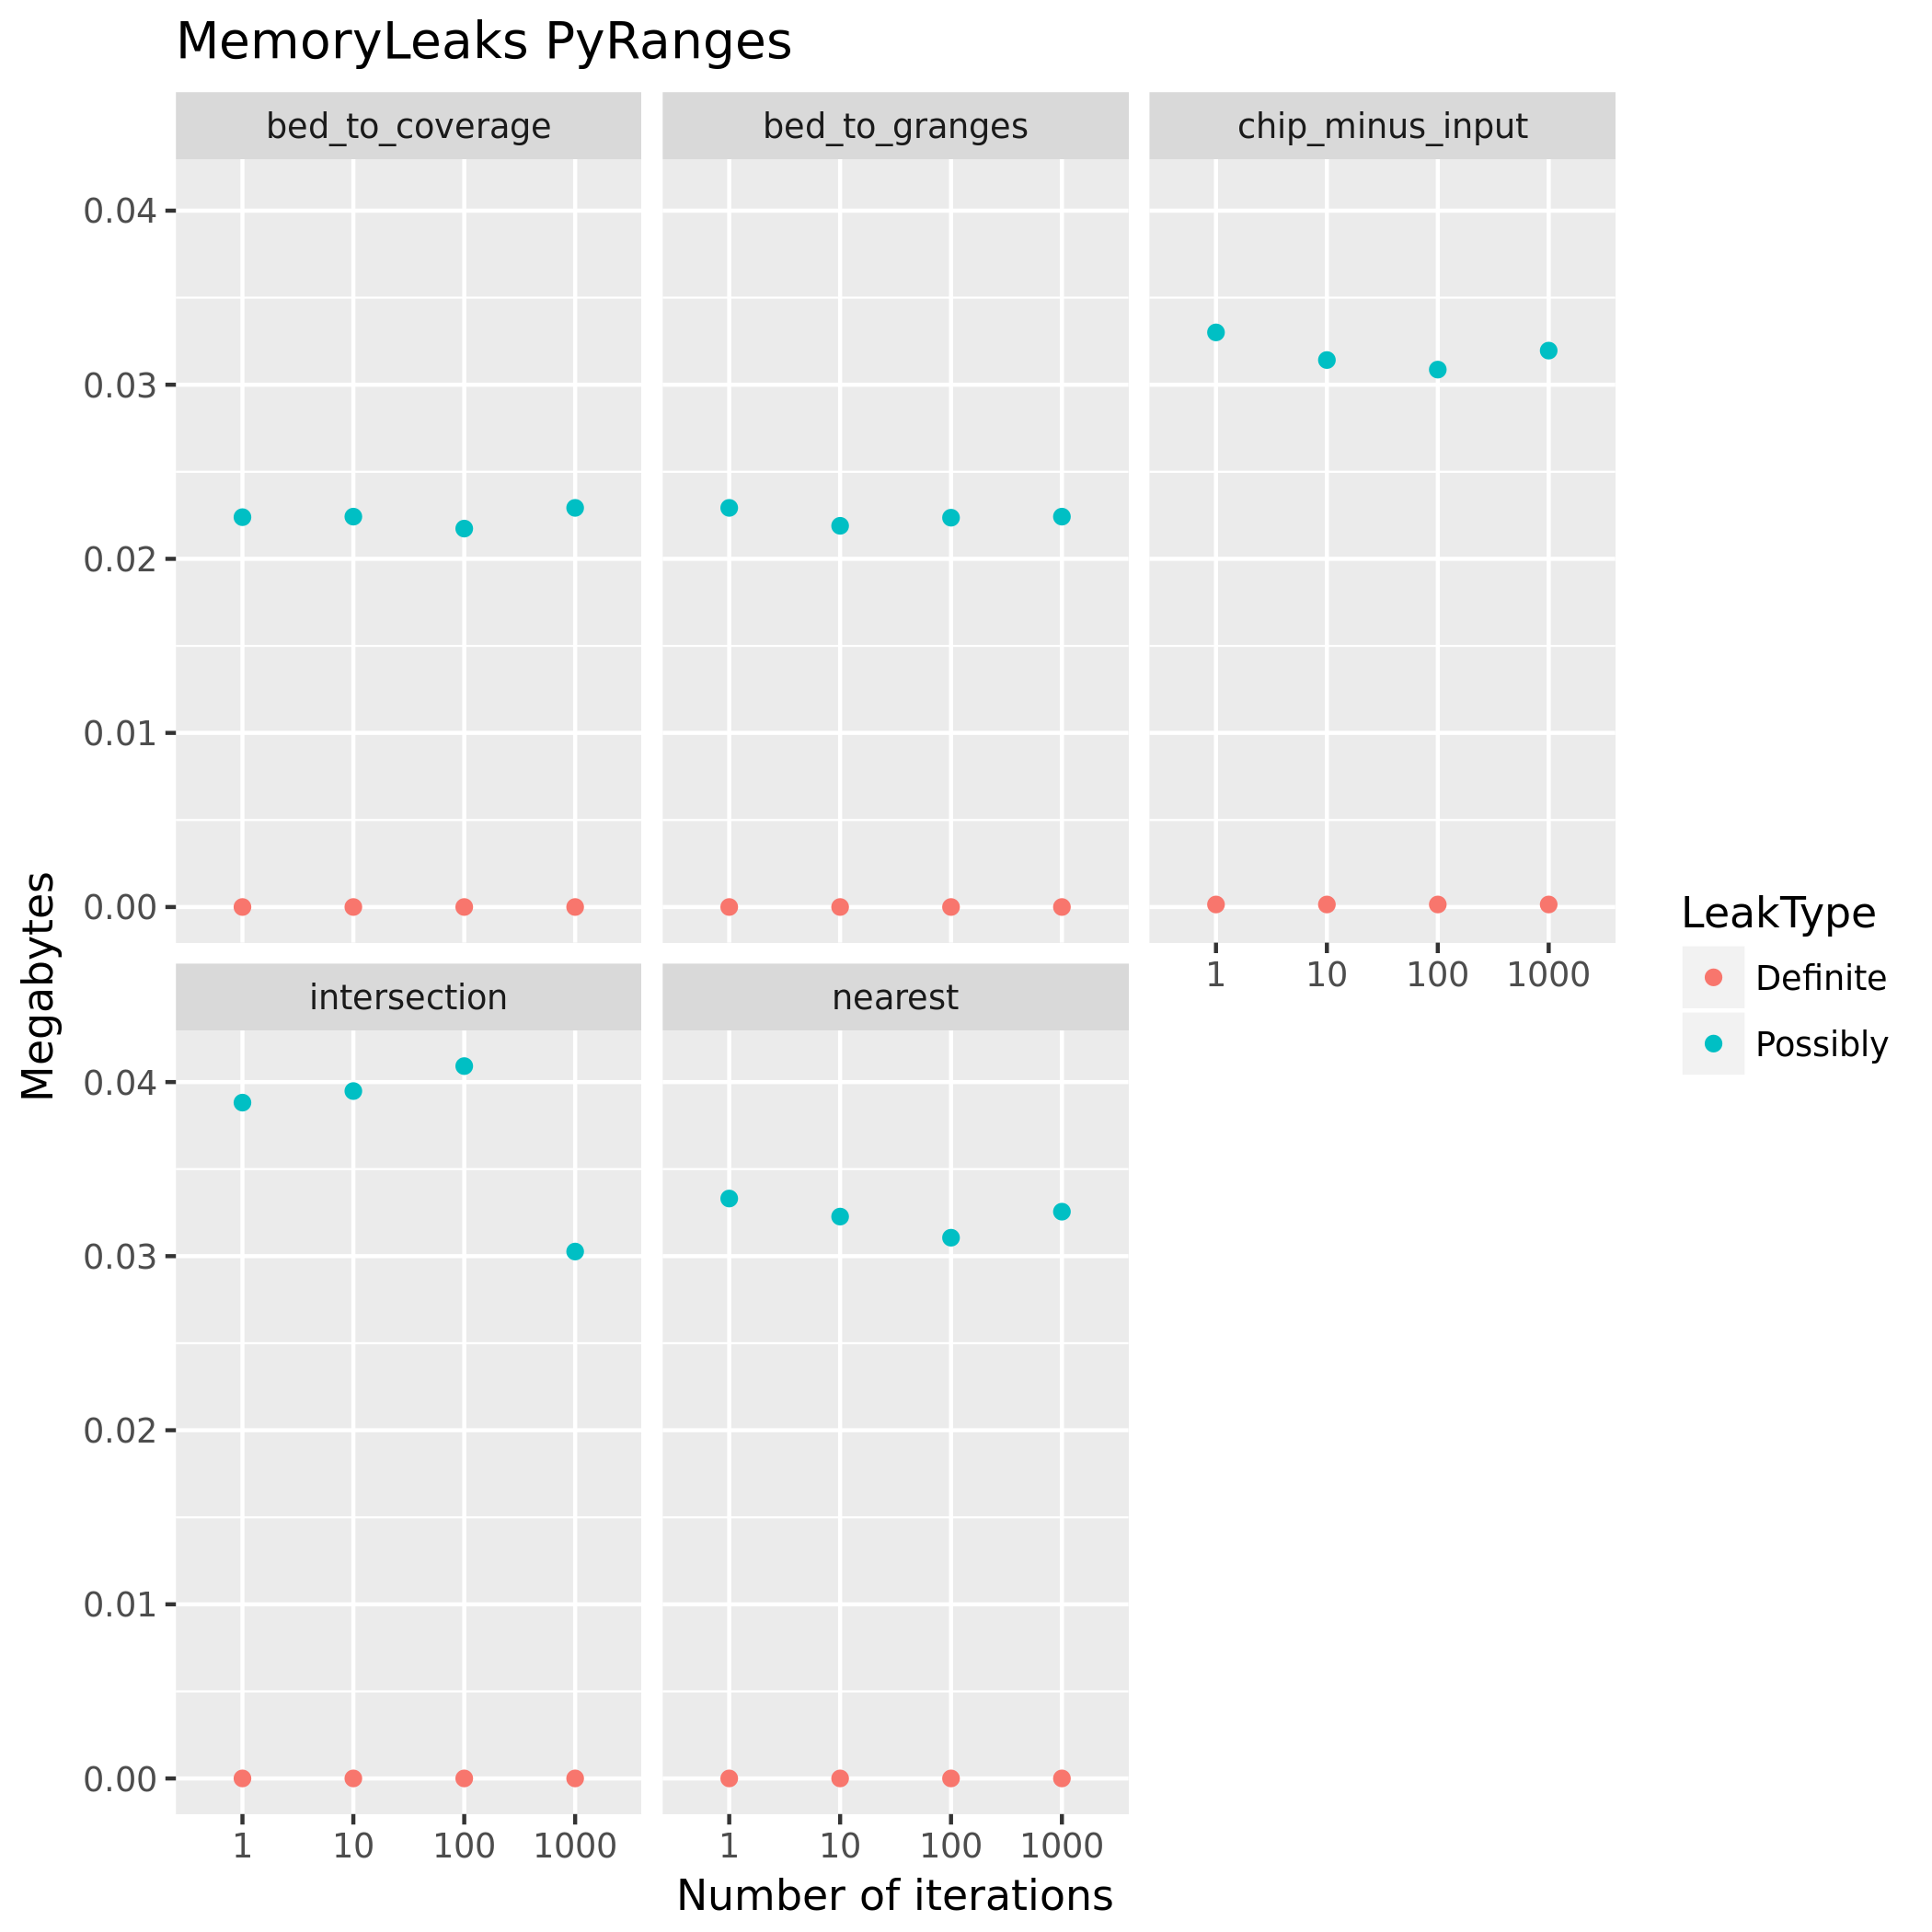
\includegraphics[width=1\textwidth]{graphs/memleak.png}
% \captionsetup{labelformat=empty} % makes sure dummy caption is blank
\caption{Memory leaks in megabytes incurred by different PyRanges functionality.
  Since the potential memory leaks were not increasing with the number of
  iterations, it seems unlikely that they are proper memory
  leaks.} % add dummy caption - otherwise \label won't work and figure numbering will not count up
\label{fig1} % use \ref{fig1} to reference to this figure
\end{figure} % avoid blank space here

\section*{Memory usage}

Memory usage of the PyRanges library was tested using the benchmarking
capabilities of Snakemake \cite{doi:10.1093/bioinformatics/bty350}. It works by
polling the running process, which means that the estimates for memory usage
also includes setup.

For most functionality, PyRanges uses a bit less memory than GenomicRanges. The
only cases where PyRanges uses more memory is for rle arithmetic and nearest,
where PyRanges leverages this memory to make the operations more than twice as
fast as R GenomicRanges. There is some variability in the memory usage, which is
to be expected for garbage collected languages.

\begin{figure}
% the number in [] of wrapfigure is optional and gives the number of text lines that should be wrapped around the text. Adjust according to your figures height
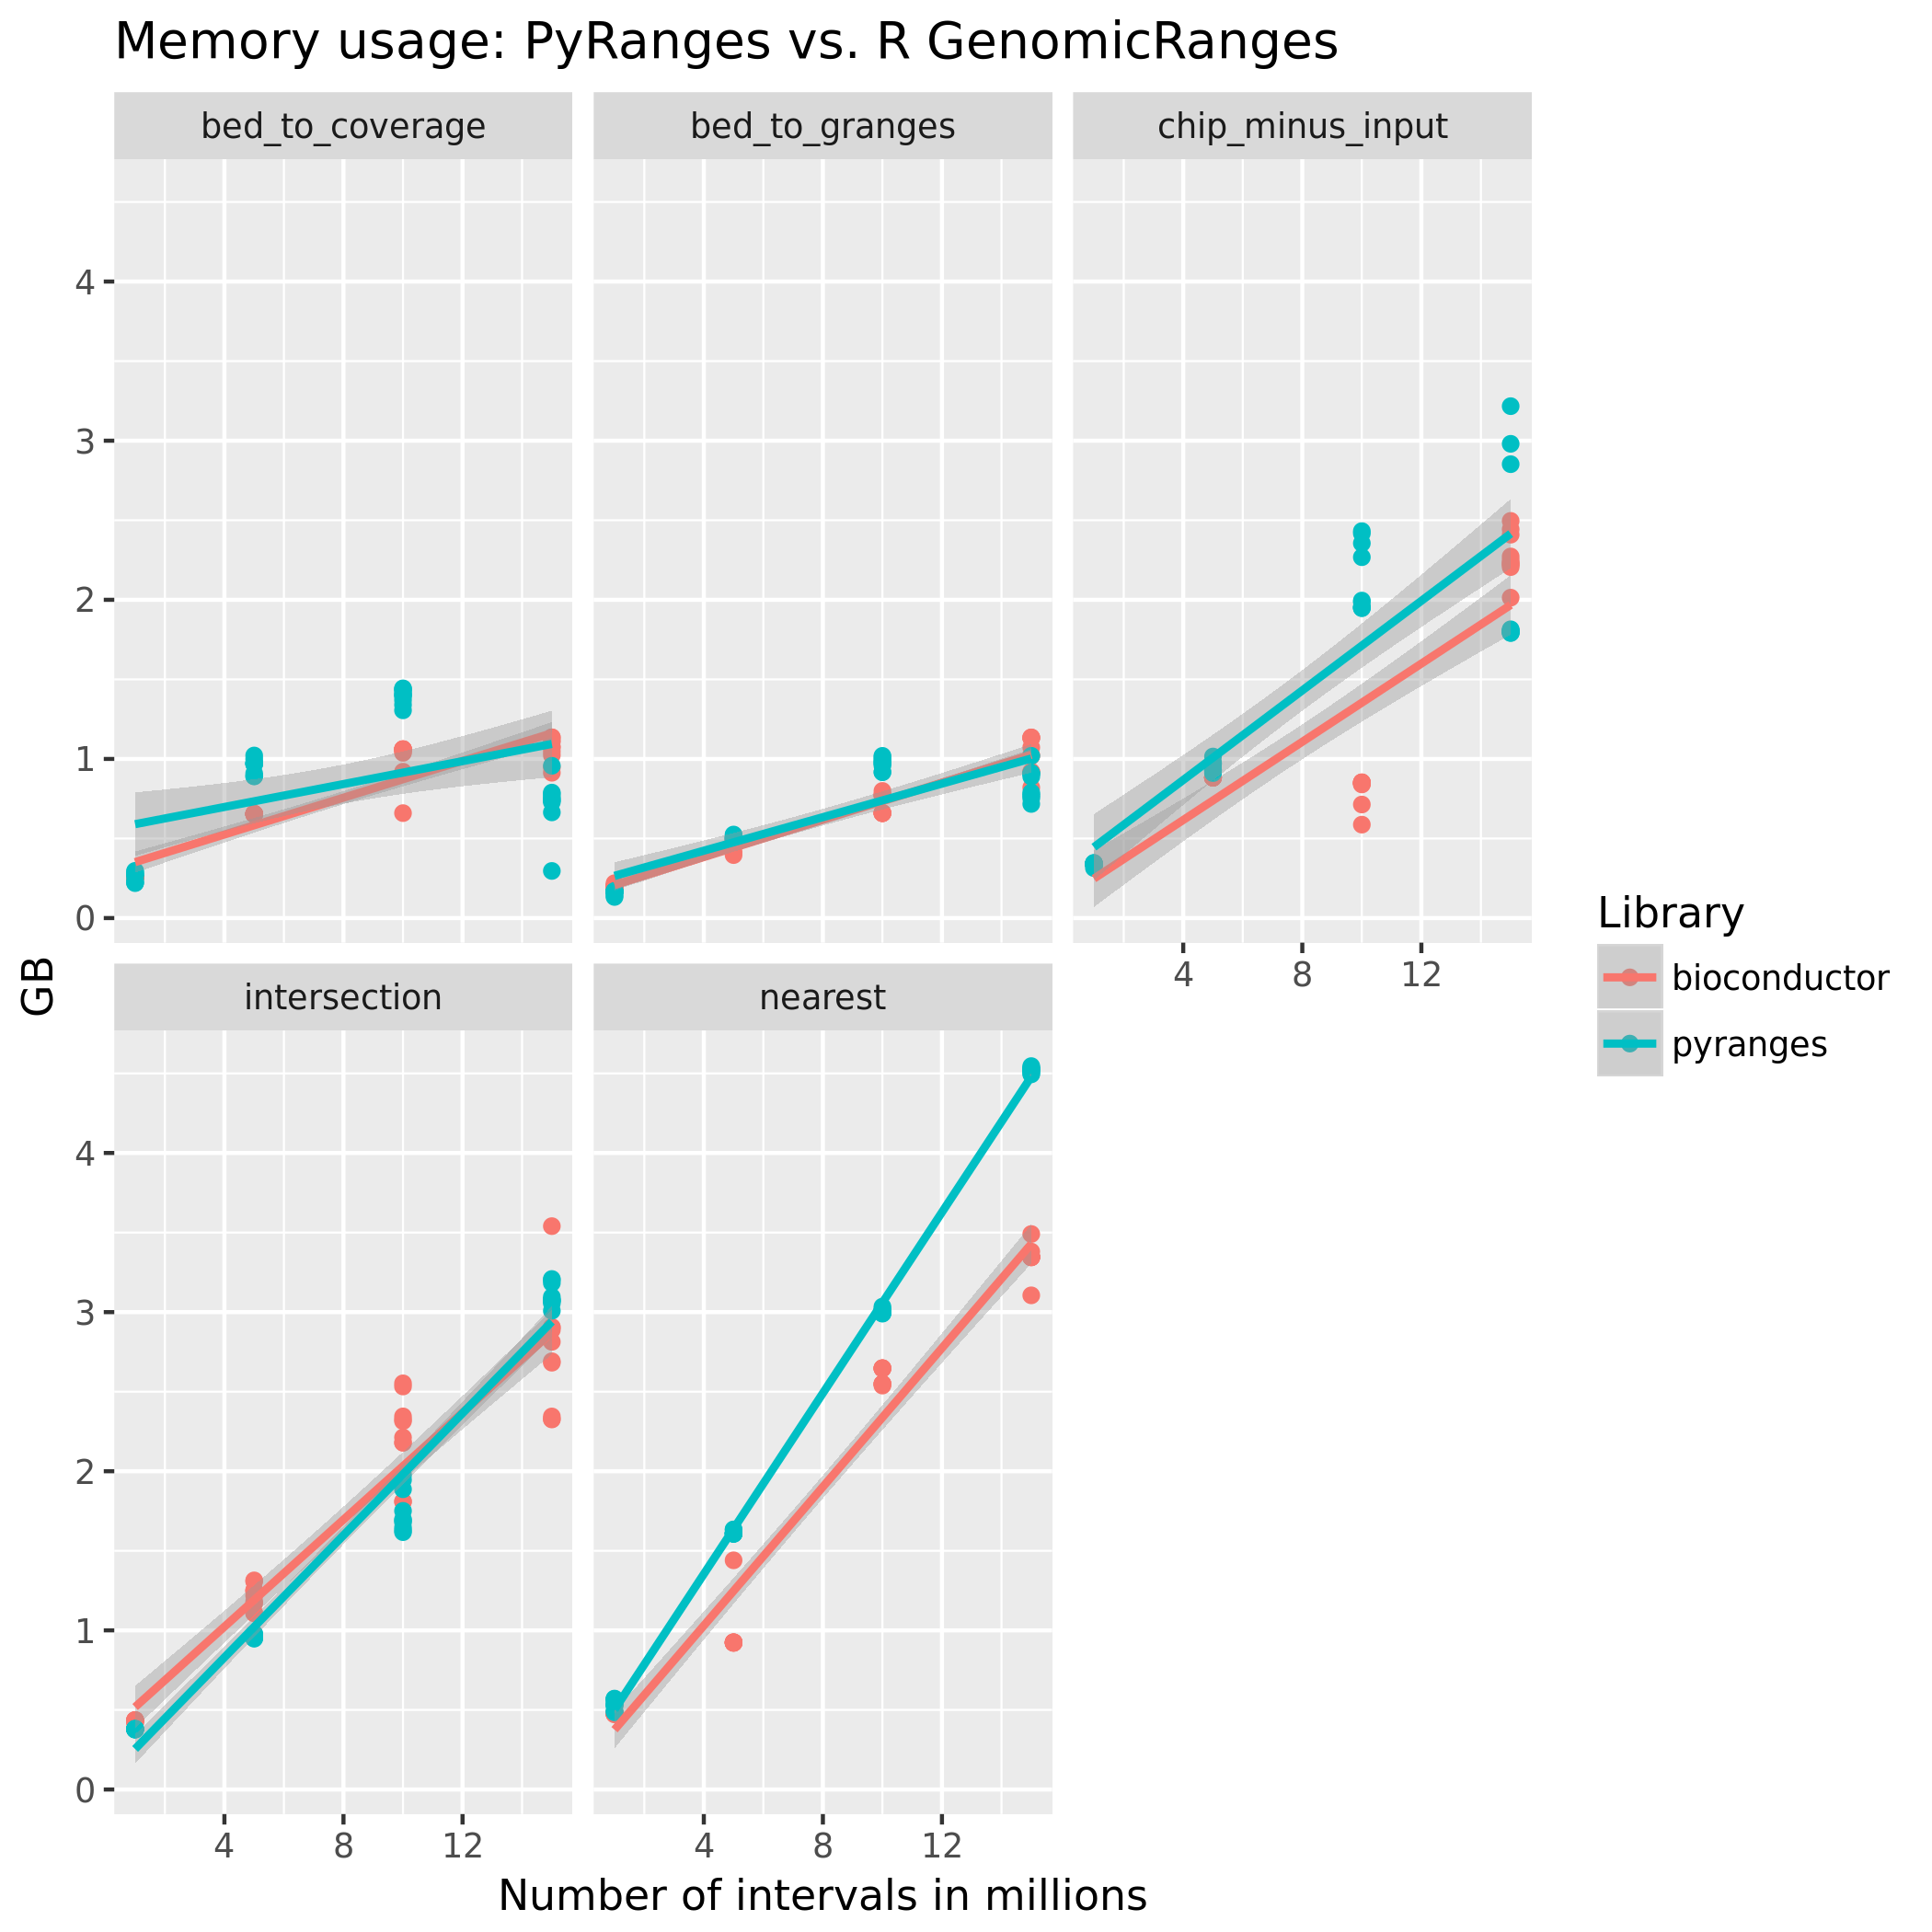
\includegraphics[width=1\textwidth]{graphs/memory.png}
% \captionsetup{labelformat=empty} % makes sure dummy caption is blank
\caption{Memory usage in GigaBytes: PyRanges vs GenomicRanges} % add dummy caption - otherwise \label won't work and figure numbering will not count up
\label{fig1} % use \ref{fig1} to reference to this figure
\end{figure} % avoid blank space here

\pagebreak
\section*{Functionality}

\begin{table}[!ht]
\begin{adjustwidth}{-1.5in}{0in}
\centering
\caption{{\bf Functionality.} Methods available on PyRanges objects.}
\begin{tabular}{|l|l|l|l|l|l|l|}
\hline
  {\bf Method} & {\bf Purpose} \\ \hline
  Subset & Use Python's getitem operator to efficiently subset PyRanges \\ \hline
  Intersection & For each feature in self, keep those that overlap with intervals in other \footnotemark \\ \hline
  Set Intersection & Treat the intervals in each PyRanges as a set and find the intersection \footnotemark \\ \hline
  Overlap & Keep each feature in self that overlaps with at least one in other \\ \hline
  Set Union & Treat the intervals in each PyRanges as a set and find the union \\ \hline
  Subtract & For each feature in self, keep those parts that do not overlap with any feature in other \\ \hline
  Set Subtract & Treat the intervals in each PyRanges as a set and subtract other from self \\ \hline
  Nearest & For each feature in self, find the nearest in other \\ \hline
  Cluster & Merge the overlapping features in a PyRanges object \\ \hline
  Coverage & Create a dictionary of run length encodings from the PyRanges object \\ \hline
\end{tabular}
\label{tab1}
\end{adjustwidth}
\end{table}

\footnotetext{Like bedtools intersect}
\footnotetext{Like BioConductor GenomicRanges intersect}

\section*{Example Usage}

\begin{adjustwidth}{-2in}{0in}
\begin{flushright}
\begin{lstlisting}[language=Python, linewidth=30cm, basicstyle=\small]
  import pyranges as pr
  from pyranges import PyRanges

  > gr1 = pr.read_bed('f1.bed')

  +--------------+---------+-------+--------+---------+----------+
  | Chromosome   |   Start |   End | Name   |   Score | Strand   |
  |--------------+---------+-------+--------+---------+----------|
  | chr1         |       3 |     6 | h      |       0 | +        |
  | chr1         |       5 |     7 | h      |       0 | -        |
  | chr1         |       8 |     9 | h      |       0 | +        |
  +--------------+---------+-------+--------+---------+----------+
  PyRanges object has 3 sequences from 1 chromosomes.

  > gr2 = pr.read_bed('f2.bed')

  +--------------+---------+-------+--------+---------+----------+
  | Chromosome   |   Start |   End | Name   |   Score | Strand   |
  |--------------+---------+-------+--------+---------+----------|
  | chr1         |       1 |     2 | f      |       0 | +        |
  | chr1         |       6 |     7 | f      |       0 | -        |
  +--------------+---------+-------+--------+---------+----------+
  PyRanges object has 2 sequences from 1 chromosomes.

  > n = gr1.nearest(gr2, strandedness="opposite", overlapping=False, suffix='_')

  # The PyRanges data can be accessed with .df
  > n.df[["Chromosome", "Start", "End", "Strand", "Start_", "End_", "Strand_", "Distance"]]

    Chromosome  Start  End Strand  Start_  End_ Strand_  Distance
  0       chr1      3    6      +       6     7       -         1
  1       chr1      8    9      +       6     7       -         2
  2       chr1      5    7      -       1     2       +         4

  # Easily create new PyRanges from a df

  > PyRanges(n.df[["Chromosome", "Start", "End", "Strand", "Start_", "End_", "Strand_", "Distance"]])

  +--------------+---------+-------+----------+----------+--------+-----------+------------+
  | Chromosome   |   Start |   End | Strand   |   Start_ |   End_ | Strand_   |   Distance |
  |--------------+---------+-------+----------+----------+--------+-----------+------------|
  | chr1         |       3 |     6 | +        |        6 |      7 | -         |          1 |
  | chr1         |       8 |     9 | +        |        6 |      7 | -         |          2 |
  | chr1         |       5 |     7 | -        |        1 |      2 | +         |          4 |
  +--------------+---------+-------+----------+----------+--------+-----------+------------+
  PyRanges object has 3 sequences from 1 chromosomes.

  > gr1.intersection(gr2)

  +--------------+---------+-------+--------+---------+----------+
  | Chromosome   |   Start |   End | Name   |   Score | Strand   |
  |--------------+---------+-------+--------+---------+----------|
  | chr1         |       6 |     7 | h      |       0 | -        |
  +--------------+---------+-------+--------+---------+----------+
  PyRanges object has 1 sequences from 1 chromosomes.

  > c = gr1.cluster()
  > c

  +--------------+---------+-------+
  | Chromosome   |   Start |   End |
  |--------------+---------+-------|
  | chr1         |       3 |     7 |
  | chr1         |       8 |     9 |
  +--------------+---------+-------+
  PyRanges object has 2 sequences from 1 chromosomes.

  > c.df.insert(3, 'ID', ["A", "B"])
  > c

  +--------------+---------+-------+------+
  | Chromosome   |   Start |   End | ID   |
  |--------------+---------+-------+------|
  | chr1         |       3 |     7 | A    |
  | chr1         |       8 |     9 | B    |
  +--------------+---------+-------+------+
  PyRanges object has 2 sequences from 1 chromosomes.

  > cv1 = gr1.coverage(strand=True)
  > cv1

  chr1 +
  --
  +--------+-----+-----+-----+-----+
  | Runs   |   3 |   3 |   2 |   1 |
  |--------+-----+-----+-----+-----|
  | Values |   0 |   1 |   0 |   1 |
  +--------+-----+-----+-----+-----+
  Rle of length 9 containing 4 elements

  chr1 -
  --
  +--------+-----+-----+
  | Runs   |   5 |   2 |
  |--------+-----+-----|
  | Values |   0 |   1 |
  +--------+-----+-----+
  Rle of length 7 containing 2 elements
  PyRles object with 2 chromosomes/strand pairs.

  > cv2 = gr2.coverage(strand=True)
  > cv2

  chr1 +
  --
  +--------+-----+-----+
  | Runs   |   1 |   1 |
  |--------+-----+-----|
  | Values |   0 |   1 |
  +--------+-----+-----+
  Rle of length 2 containing 2 elements

  chr1 -
  --
  +--------+-----+-----+
  | Runs   |   6 |   1 |
  |--------+-----+-----|
  | Values |   0 |   1 |
  +--------+-----+-----+
  Rle of length 7 containing 2 elements
  PyRles object with 2 chromosomes/strand pairs.

  > cv1 - cv2

    chr1 +
  --
  +--------+-----+-----+-----+-----+-----+-----+
  | Runs   |   1 |   1 |   1 |   3 |   2 |   1 |
  |--------+-----+-----+-----+-----+-----+-----|
  | Values |   0 |  -1 |   0 |   1 |   0 |   1 |
  +--------+-----+-----+-----+-----+-----+-----+
  Rle of length 9 containing 6 elements

  chr1 -
  --
  +--------+-----+-----+-----+
  | Runs   |   5 |   1 |   1 |
  |--------+-----+-----+-----|
  | Values |   0 |   1 |   0 |
  +--------+-----+-----+-----+
  Rle of length 7 containing 3 elements
  PyRles object with 2 chromosomes/strand pairs.

\end{lstlisting}
\end{flushright}

\end{adjustwidth}



\bibliographystyle{abbrv}

\bibliography{library}
\end{document}
